% Options for packages loaded elsewhere
\PassOptionsToPackage{unicode}{hyperref}
\PassOptionsToPackage{hyphens}{url}
\PassOptionsToPackage{dvipsnames,svgnames,x11names}{xcolor}
%
\documentclass[
  letterpaper,
  DIV=11,
  numbers=noendperiod]{scrartcl}

\usepackage{amsmath,amssymb}
\usepackage{iftex}
\ifPDFTeX
  \usepackage[T1]{fontenc}
  \usepackage[utf8]{inputenc}
  \usepackage{textcomp} % provide euro and other symbols
\else % if luatex or xetex
  \usepackage{unicode-math}
  \defaultfontfeatures{Scale=MatchLowercase}
  \defaultfontfeatures[\rmfamily]{Ligatures=TeX,Scale=1}
\fi
\usepackage{lmodern}
\ifPDFTeX\else  
    % xetex/luatex font selection
\fi
% Use upquote if available, for straight quotes in verbatim environments
\IfFileExists{upquote.sty}{\usepackage{upquote}}{}
\IfFileExists{microtype.sty}{% use microtype if available
  \usepackage[]{microtype}
  \UseMicrotypeSet[protrusion]{basicmath} % disable protrusion for tt fonts
}{}
\makeatletter
\@ifundefined{KOMAClassName}{% if non-KOMA class
  \IfFileExists{parskip.sty}{%
    \usepackage{parskip}
  }{% else
    \setlength{\parindent}{0pt}
    \setlength{\parskip}{6pt plus 2pt minus 1pt}}
}{% if KOMA class
  \KOMAoptions{parskip=half}}
\makeatother
\usepackage{xcolor}
\setlength{\emergencystretch}{3em} % prevent overfull lines
\setcounter{secnumdepth}{5}
% Make \paragraph and \subparagraph free-standing
\makeatletter
\ifx\paragraph\undefined\else
  \let\oldparagraph\paragraph
  \renewcommand{\paragraph}{
    \@ifstar
      \xxxParagraphStar
      \xxxParagraphNoStar
  }
  \newcommand{\xxxParagraphStar}[1]{\oldparagraph*{#1}\mbox{}}
  \newcommand{\xxxParagraphNoStar}[1]{\oldparagraph{#1}\mbox{}}
\fi
\ifx\subparagraph\undefined\else
  \let\oldsubparagraph\subparagraph
  \renewcommand{\subparagraph}{
    \@ifstar
      \xxxSubParagraphStar
      \xxxSubParagraphNoStar
  }
  \newcommand{\xxxSubParagraphStar}[1]{\oldsubparagraph*{#1}\mbox{}}
  \newcommand{\xxxSubParagraphNoStar}[1]{\oldsubparagraph{#1}\mbox{}}
\fi
\makeatother


\providecommand{\tightlist}{%
  \setlength{\itemsep}{0pt}\setlength{\parskip}{0pt}}\usepackage{longtable,booktabs,array}
\usepackage{calc} % for calculating minipage widths
% Correct order of tables after \paragraph or \subparagraph
\usepackage{etoolbox}
\makeatletter
\patchcmd\longtable{\par}{\if@noskipsec\mbox{}\fi\par}{}{}
\makeatother
% Allow footnotes in longtable head/foot
\IfFileExists{footnotehyper.sty}{\usepackage{footnotehyper}}{\usepackage{footnote}}
\makesavenoteenv{longtable}
\usepackage{graphicx}
\makeatletter
\def\maxwidth{\ifdim\Gin@nat@width>\linewidth\linewidth\else\Gin@nat@width\fi}
\def\maxheight{\ifdim\Gin@nat@height>\textheight\textheight\else\Gin@nat@height\fi}
\makeatother
% Scale images if necessary, so that they will not overflow the page
% margins by default, and it is still possible to overwrite the defaults
% using explicit options in \includegraphics[width, height, ...]{}
\setkeys{Gin}{width=\maxwidth,height=\maxheight,keepaspectratio}
% Set default figure placement to htbp
\makeatletter
\def\fps@figure{htbp}
\makeatother
% definitions for citeproc citations
\NewDocumentCommand\citeproctext{}{}
\NewDocumentCommand\citeproc{mm}{%
  \begingroup\def\citeproctext{#2}\cite{#1}\endgroup}
\makeatletter
 % allow citations to break across lines
 \let\@cite@ofmt\@firstofone
 % avoid brackets around text for \cite:
 \def\@biblabel#1{}
 \def\@cite#1#2{{#1\if@tempswa , #2\fi}}
\makeatother
\newlength{\cslhangindent}
\setlength{\cslhangindent}{1.5em}
\newlength{\csllabelwidth}
\setlength{\csllabelwidth}{3em}
\newenvironment{CSLReferences}[2] % #1 hanging-indent, #2 entry-spacing
 {\begin{list}{}{%
  \setlength{\itemindent}{0pt}
  \setlength{\leftmargin}{0pt}
  \setlength{\parsep}{0pt}
  % turn on hanging indent if param 1 is 1
  \ifodd #1
   \setlength{\leftmargin}{\cslhangindent}
   \setlength{\itemindent}{-1\cslhangindent}
  \fi
  % set entry spacing
  \setlength{\itemsep}{#2\baselineskip}}}
 {\end{list}}
\usepackage{calc}
\newcommand{\CSLBlock}[1]{\hfill\break\parbox[t]{\linewidth}{\strut\ignorespaces#1\strut}}
\newcommand{\CSLLeftMargin}[1]{\parbox[t]{\csllabelwidth}{\strut#1\strut}}
\newcommand{\CSLRightInline}[1]{\parbox[t]{\linewidth - \csllabelwidth}{\strut#1\strut}}
\newcommand{\CSLIndent}[1]{\hspace{\cslhangindent}#1}

\KOMAoption{captions}{tableheading}
\makeatletter
\@ifpackageloaded{caption}{}{\usepackage{caption}}
\AtBeginDocument{%
\ifdefined\contentsname
  \renewcommand*\contentsname{Table of contents}
\else
  \newcommand\contentsname{Table of contents}
\fi
\ifdefined\listfigurename
  \renewcommand*\listfigurename{List of Figures}
\else
  \newcommand\listfigurename{List of Figures}
\fi
\ifdefined\listtablename
  \renewcommand*\listtablename{List of Tables}
\else
  \newcommand\listtablename{List of Tables}
\fi
\ifdefined\figurename
  \renewcommand*\figurename{Figure}
\else
  \newcommand\figurename{Figure}
\fi
\ifdefined\tablename
  \renewcommand*\tablename{Table}
\else
  \newcommand\tablename{Table}
\fi
}
\@ifpackageloaded{float}{}{\usepackage{float}}
\floatstyle{ruled}
\@ifundefined{c@chapter}{\newfloat{codelisting}{h}{lop}}{\newfloat{codelisting}{h}{lop}[chapter]}
\floatname{codelisting}{Listing}
\newcommand*\listoflistings{\listof{codelisting}{List of Listings}}
\makeatother
\makeatletter
\makeatother
\makeatletter
\@ifpackageloaded{caption}{}{\usepackage{caption}}
\@ifpackageloaded{subcaption}{}{\usepackage{subcaption}}
\makeatother

\ifLuaTeX
  \usepackage{selnolig}  % disable illegal ligatures
\fi
\usepackage{bookmark}

\IfFileExists{xurl.sty}{\usepackage{xurl}}{} % add URL line breaks if available
\urlstyle{same} % disable monospaced font for URLs
\hypersetup{
  pdftitle={My title},
  pdfauthor={Lexun Yu},
  colorlinks=true,
  linkcolor={blue},
  filecolor={Maroon},
  citecolor={Blue},
  urlcolor={Blue},
  pdfcreator={LaTeX via pandoc}}


\title{My title\thanks{Code and data are available at:
\url{https://github.com/yulexun/toronto-fire}.}}
\usepackage{etoolbox}
\makeatletter
\providecommand{\subtitle}[1]{% add subtitle to \maketitle
  \apptocmd{\@title}{\par {\large #1 \par}}{}{}
}
\makeatother
\subtitle{My subtitle if needed}
\author{Lexun Yu}
\date{September 22, 2024}

\begin{document}
\maketitle
\begin{abstract}
First sentence. Second sentence. Third sentence. Fourth sentence.
\end{abstract}

\renewcommand*\contentsname{Table of contents}
{
\hypersetup{linkcolor=}
\setcounter{tocdepth}{3}
\tableofcontents
}

\section{Introduction}\label{sec-intro}

The urban fire hazard is one of the most pressing issues in this
context, especially in Canada where cities are dealing with such issues
like climate, facilities or population density.As of July 1 2023, the
population in urban area in Canada reached 33,812,133 (Statistics Canada
2024). Not only do fires in highly populated regions result in heavy
losses in terms of property, but also, in the contest of people and the
environment, the consequences are enormous. Also, urban fires are
resources-dependent and require attention from city services and
emergency services, thus indicating the need for prevention, action and
planning based on risk assessment. With such issues in mind, the
knowledge of urban fire hazards in Canadian cities is needed for
creating policies that address public safety and increase urban
resilience.

In Canada, articles about fire incidents has a focus on wildfire. For
instance, Goemans and Ballamingie (2012) discuss the fire mitigation
plan during the 2003 wildfire at Kelowna, British Columbia, while Mamuji
and Rozdilsky (2018) talk about the evacuation during the Fort McMurray
wildfire in Alberta. The researches conducted about urban fire incidents
are done in other parts of the world such as East Asia. Masood Rafi,
Wasiuddin, and Hameed Siddiqui (2012) research the nature and level of
this threat. They conclude that the lack of training in fire department,
shortage of facilities and infrastructure the major issues in Pakistan.
The research by Hari Murti et al. (2023) in Semarang City also emphasize
the importance of community understanding and the installation of fire
protection facilities. This article uses the data provided by
opendatatoronto library (Gelfand 2022) in order to analyze fire
occurrences in the city of Toronto, which is an important research gap
in the study of fire incidents in America. This study seeks to provide a
deeper understanding of fire patterns to improve fire prevention and
emergency response strategies.

In this paper we visualize Toronto's Fire Incidents data.

\section{Data}\label{data}

\subsection{Overview}\label{sec-data-overview}

The data used in this paper is obtained from the opendatatoronto library
(Gelfand 2022). The dataset used is Fire Incidents. According to Gelfand
(2022), it includes fire incidents as defined by the Ontario Fire
Marshal (OFM) up to December 31, 2023. The data gathering and analysis
is done in R (R Core Team 2024) with the following packages:
opendatatoronto (Gelfand 2022), knitr (Xie 2014), tidyverse (Wickham et
al. 2019), ggplot2 (Wickham 2016), dplyr (Wickham et al. 2023), and
lubridate (Grolemund and Wickham 2011).

The cleaned data are divided into two groups in accordance to the two
most important factors in urban fire incidents: responsiveness of fire
department and fire protection equipments, as indicated by Hari Murti et
al. (2023) and Masood Rafi, Wasiuddin, and Hameed Siddiqui (2012). The
first group focuses on the fire services' response time, extent of fire
and the loss of money, and the second group focuses on the loss of
money, reason of fire incidents and the presence or operation of fire
protection equipments. All other data features are ignored during the
data cleaning process.

\subsection{Toronto Fire Service
Responsiveness}\label{toronto-fire-service-responsiveness}

The first group of data shows the responsiveness of Toronto Fire
Services. An example of this dataset is presented in
Table~\ref{tbl-clean-tfs}. ``Alarm Time'' is the time when TFS are
notified of the incident. ``TFS Arrival time'' is the timestamp of first
arriving unit. The difference in minute is calculated at the data
cleaning step as ``TFS Response Time''. ``Estimated Loss in Dollar'' is
the estimated loss measured in dollar. ``Extent of Fire'' is a
categorical indicator from ``1'' to ``11'' according to the seriousness
of the incident.

\begin{longtable}[]{@{}
  >{\raggedright\arraybackslash}p{(\columnwidth - 8\tabcolsep) * \real{0.2041}}
  >{\raggedright\arraybackslash}p{(\columnwidth - 8\tabcolsep) * \real{0.2041}}
  >{\raggedleft\arraybackslash}p{(\columnwidth - 8\tabcolsep) * \real{0.1837}}
  >{\raggedleft\arraybackslash}p{(\columnwidth - 8\tabcolsep) * \real{0.2551}}
  >{\raggedleft\arraybackslash}p{(\columnwidth - 8\tabcolsep) * \real{0.1531}}@{}}

\caption{\label{tbl-clean-tfs}Top rows of cleaned Toronto Fire Service
response time and loss data}

\tabularnewline

\toprule\noalign{}
\begin{minipage}[b]{\linewidth}\raggedright
Alarm Time
\end{minipage} & \begin{minipage}[b]{\linewidth}\raggedright
TFS Arrival Time
\end{minipage} & \begin{minipage}[b]{\linewidth}\raggedleft
TFS Response Time
\end{minipage} & \begin{minipage}[b]{\linewidth}\raggedleft
Estimated Loss in Dollar
\end{minipage} & \begin{minipage}[b]{\linewidth}\raggedleft
Extent of Fire
\end{minipage} \\
\midrule\noalign{}
\endhead
\bottomrule\noalign{}
\endlastfoot
2018-02-25 15:48:34 & 2018-02-25 15:52:04 & 3.500000 & 5000 & 1 \\
2018-02-26 18:11:59 & 2018-02-26 18:15:50 & 3.850000 & 500 & 1 \\
2018-03-03 09:49:14 & 2018-03-03 09:53:09 & 3.916667 & 0 & 1 \\
2018-03-03 17:54:38 & 2018-03-03 17:59:42 & 5.066667 & 15000 & 2 \\
2018-03-03 18:34:35 & 2018-03-03 18:40:47 & 6.200000 & 0 & 1 \\

\end{longtable}

Figure~\ref{fig-clean-tfs-diff-dollar-time-1} shows the line plot of
Toronto Fire Service's response time over the period between 2013 to
2023. The response time fluctuated around a relatively consistent level,
typically between 5 and 10 minutes, with occasional spikes where the
response time increased significantly above the usual range,
particularly around 2014 and 2019.
Figure~\ref{fig-clean-tfs-diff-dollar-time-2} shows the line plot of
estimated dollar loss of the fire incidents. Most of the incidents
resulted in relatively low dollar losses, but there are several spikes
that represent incidents where the loss was significantly higher. Some
of the most notable spikes occurred between 2015 and 2019, with losses
exceeding 2 million dollars.

\begin{figure}

\begin{minipage}{0.50\linewidth}

\centering{

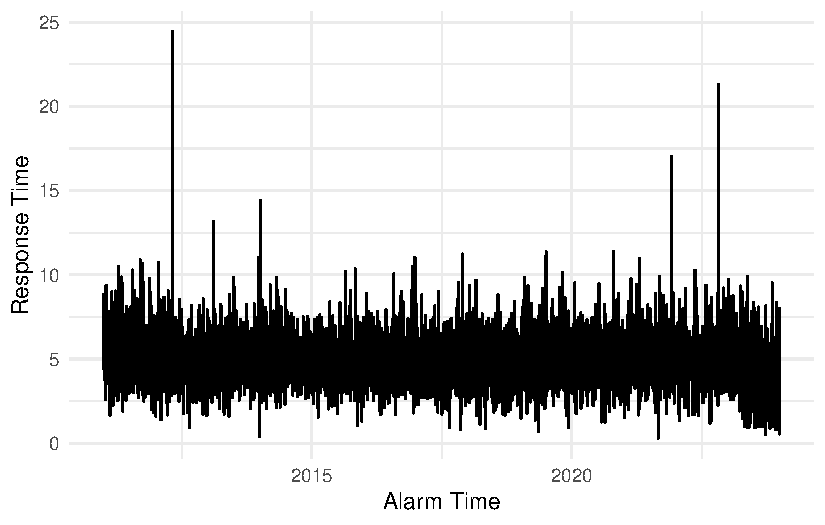
\includegraphics{paper_files/figure-pdf/fig-clean-tfs-diff-dollar-time-1.pdf}

}

\subcaption{\label{fig-clean-tfs-diff-dollar-time-1}TFS response time
over time}

\end{minipage}%
%
\begin{minipage}{0.50\linewidth}

\centering{

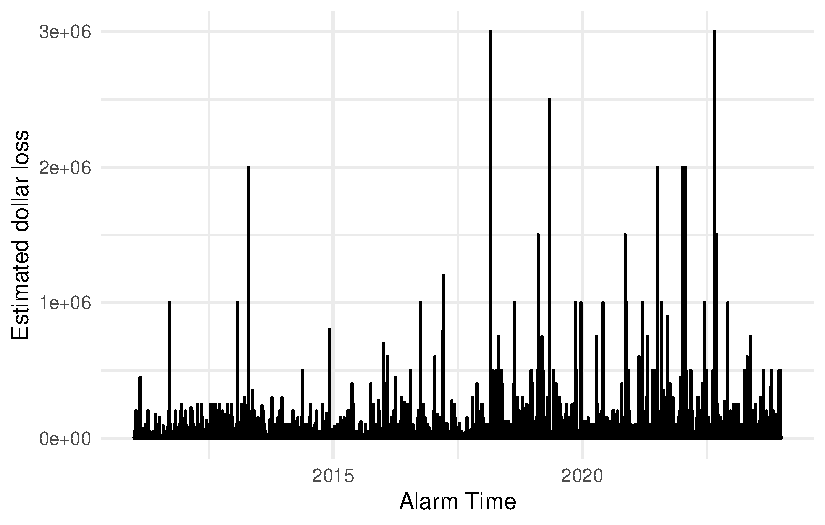
\includegraphics{paper_files/figure-pdf/fig-clean-tfs-diff-dollar-time-2.pdf}

}

\subcaption{\label{fig-clean-tfs-diff-dollar-time-2}Estimated dollar
loss over time}

\end{minipage}%

\caption{\label{fig-clean-tfs-diff-dollar-time}TFS response time and
estimated dollar loss over time}

\end{figure}%

Table~\ref{tbl-clean-tfs-summary-1} indicates the summary statistic and
Figure~\ref{fig-clean-tfs-boxplot-1} graphs the boxplot of TFS's
response time. The value mainly range from 4.03 minutes to 5.7 minutes
as shown in Table~\ref{tbl-clean-tfs-summary-1}, with a mean value of
4.911868 minutes. Notably, in Figure~\ref{fig-clean-tfs-boxplot-1},
several outliers are indicated by dots above the upper whisker,
suggesting occasional instances of significantly higher response times.

Table~\ref{tbl-clean-tfs-summary-2} indicates the summary statistic and
Figure~\ref{fig-clean-tfs-boxplot-2} depicts the distribution of
financial losses in boxplot. In Table~\ref{tbl-clean-tfs-summary-2},
values span from 0 dollar to over 3000000 dollars, with median value of
3000 dollars, mean value of 24551.64 dollars and standard deviation of
93520.08 dollars, indicating a skewed distribution.
Figure~\ref{fig-clean-tfs-boxplot-2} reveals numerous outliers above the
upper whisker, highlighting instances of exceptionally high financial
losses.

\begin{figure}

\begin{minipage}{0.50\linewidth}

\centering{

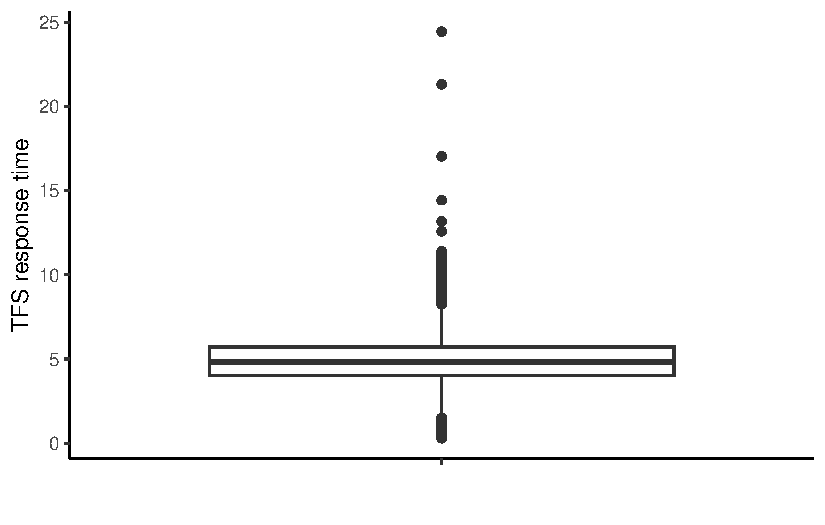
\includegraphics{paper_files/figure-pdf/fig-clean-tfs-boxplot-1.pdf}

}

\subcaption{\label{fig-clean-tfs-boxplot-1}Boxplot of TFS response time}

\end{minipage}%
%
\begin{minipage}{0.50\linewidth}

\centering{

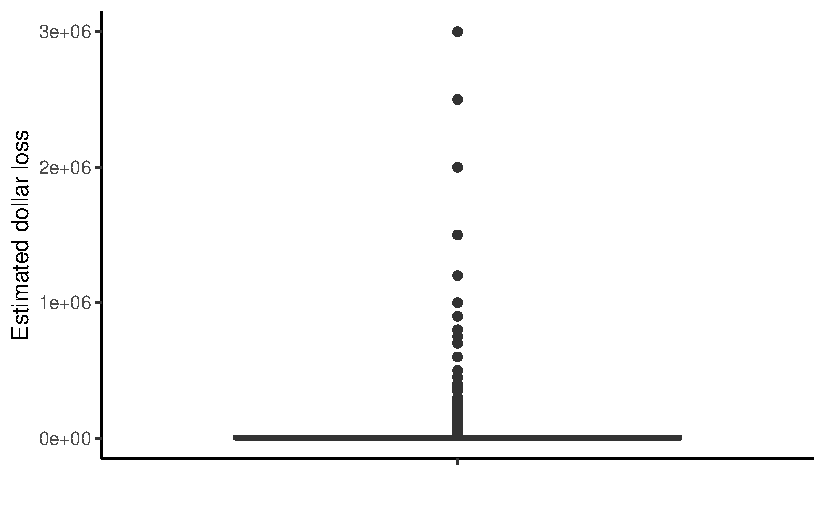
\includegraphics{paper_files/figure-pdf/fig-clean-tfs-boxplot-2.pdf}

}

\subcaption{\label{fig-clean-tfs-boxplot-2}Boxplot of estimated dollar
loss}

\end{minipage}%

\caption{\label{fig-clean-tfs-boxplot}Boxplot of TFS response time data
and estimated dollar loss}

\end{figure}%

\begin{table}

\caption{\label{tbl-clean-tfs-summary}Summary Statistic of TFS response
time data and estimated dollar loss}

\begin{minipage}{0.50\linewidth}

\subcaption{\label{tbl-clean-tfs-summary-1}Summary of TFS response time}

\centering{

\begin{tabular}{lr}
\toprule
Statistic & Value\\
\midrule
Min. & 0.300000\\
1st Qu. & 4.033333\\
Median & 4.816667\\
Mean & 4.911166\\
3rd Qu. & 5.716667\\
Max. & 24.433333\\
SD & 1.399413\\
\bottomrule
\end{tabular}

}

\end{minipage}%
%
\begin{minipage}{0.50\linewidth}

\subcaption{\label{tbl-clean-tfs-summary-2}Summary of estimated dollar loss}

\centering{

\begin{tabular}{lr}
\toprule
Statistic & Value\\
\midrule
Min. & 0.00\\
1st Qu. & 500.00\\
Median & 3000.00\\
Mean & 26584.26\\
3rd Qu. & 15000.00\\
Max. & 3000000.00\\
SD & 104422.21\\
\bottomrule
\end{tabular}

}

\end{minipage}%

\end{table}%

Figure~\ref{fig-bar-extent} illustrates that most of the observed fires
are relatively small in size. The x-axis depicts the extent of the fire,
while the y-axis shows the frequency of observations. A notably tall bar
at the start signifies a high occurrence of smaller fires. As fire size
increases along the x-axis, the number of observations drops sharply,
indicating that larger fires are far less frequent.

\begin{figure}

\centering{

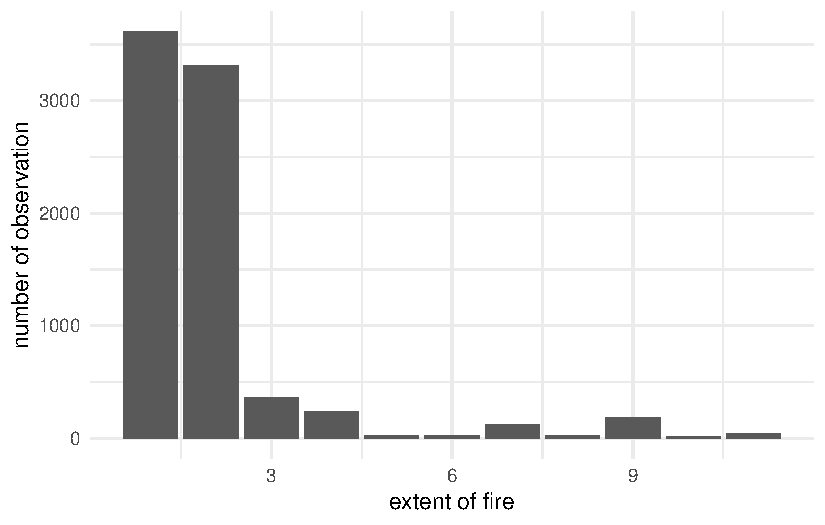
\includegraphics{paper_files/figure-pdf/fig-bar-extent-1.pdf}

}

\caption{\label{fig-bar-extent}Distribution of extent of fire}

\end{figure}%

Figure~\ref{fig-response-vs-money} shows a line of best fit, which
indicates a weak correlation between TFS response time and estimated
dollar loss. There is a wide range of TFS response times for lower
dollar losses.

\begin{figure}

\centering{

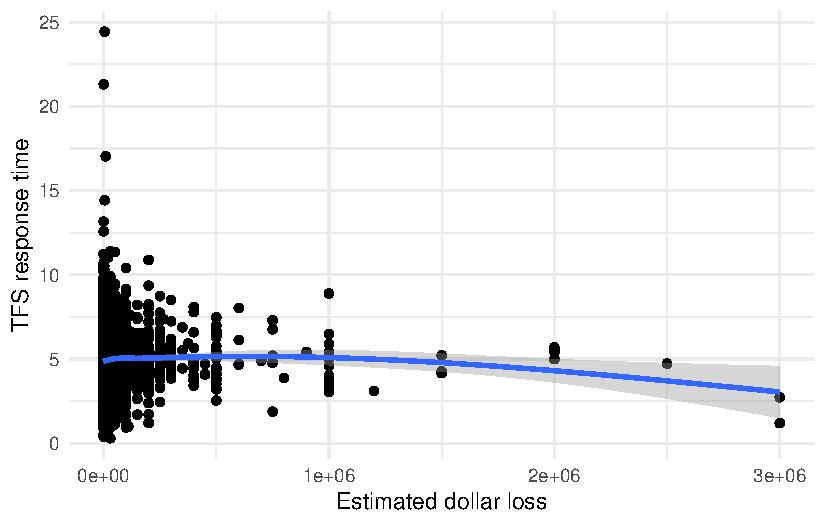
\includegraphics{paper_files/figure-pdf/fig-response-vs-money-1.pdf}

}

\caption{\label{fig-response-vs-money}Line of best fit between TFS
response time and dollar loss}

\end{figure}%

\subsection{Fire Protection
Equipments}\label{fire-protection-equipments}

The second group of data shows the money loss, cause of fire and the
presence of fire prevention equipments. Table~\ref{tbl-clean-cat} shows
the first five rows of the second group of data. ``Estimated Loss in
Dollar'' is the estimated loss measured in dollar. ``Area of origin''
indicates the area fire originate. ``Ignition Source'' shows the object
causing fire. ``Fire Alarm Status'', ``Smoke Alarm Status'' and
``Sprinkler System Status'' indicates the presence and operation of fire
protection equipments. In the second group of data, `PO' = System
present, `N' = System not present, and `P' = System present but not
operated.

\begin{longtable}[]{@{}
  >{\raggedleft\arraybackslash}p{(\columnwidth - 10\tabcolsep) * \real{0.2137}}
  >{\raggedright\arraybackslash}p{(\columnwidth - 10\tabcolsep) * \real{0.1282}}
  >{\raggedright\arraybackslash}p{(\columnwidth - 10\tabcolsep) * \real{0.1368}}
  >{\raggedright\arraybackslash}p{(\columnwidth - 10\tabcolsep) * \real{0.1538}}
  >{\raggedright\arraybackslash}p{(\columnwidth - 10\tabcolsep) * \real{0.1624}}
  >{\raggedright\arraybackslash}p{(\columnwidth - 10\tabcolsep) * \real{0.2051}}@{}}

\caption{\label{tbl-clean-cat}Top rows of cleaned data showing Area of
Origin, Ignition source and Fire, Smoke, Sprnkler System Presence.}

\tabularnewline

\toprule\noalign{}
\begin{minipage}[b]{\linewidth}\raggedleft
Estimated Loss in Dollar
\end{minipage} & \begin{minipage}[b]{\linewidth}\raggedright
Area of Origin
\end{minipage} & \begin{minipage}[b]{\linewidth}\raggedright
Ignition Source
\end{minipage} & \begin{minipage}[b]{\linewidth}\raggedright
Fire Alarm Status
\end{minipage} & \begin{minipage}[b]{\linewidth}\raggedright
Smoke Alarm Status
\end{minipage} & \begin{minipage}[b]{\linewidth}\raggedright
Sprinkler System Status
\end{minipage} \\
\midrule\noalign{}
\endhead
\bottomrule\noalign{}
\endlastfoot
5000 & 28 & 41 & P & PO & P \\
500 & 24 & 11 & P & PO & N \\
0 & 24 & 11 & N & PO & P \\
15000 & 25 & 24 & N & N & N \\
0 & 24 & 11 & P & PO & P \\

\end{longtable}

Figure~\ref{fig-origin} in \hyperref[sec-origin-fig]{Appendix A.1}
illustrates the distribution of the fire incidents' area of origin. It
consists 71 unique categories. The most common area of origin is
category 24, which is cooking area or kitchen. Other common areas
include category 64: Porch or Balcony, 22: Sleeping Area or Bedroom, 21:
Living Area, and 27: Laundry Area. However, fires in these locations
occur significantly less often compared to those in kitchens.

Figure~\ref{fig-source} in \hyperref[sec-source-fig]{Appendix A.2} shows
the distribution of ignition source in fire incidents. It contains 73
unique categories. The most common ignition source is 11: Stove,
Range-top burner and 71: Smoker's Articles. Other common ignition
sources include 55: Candle, 43: Clothes Dryer, and 12: Oven.

\begin{figure}

\begin{minipage}{0.50\linewidth}

\centering{

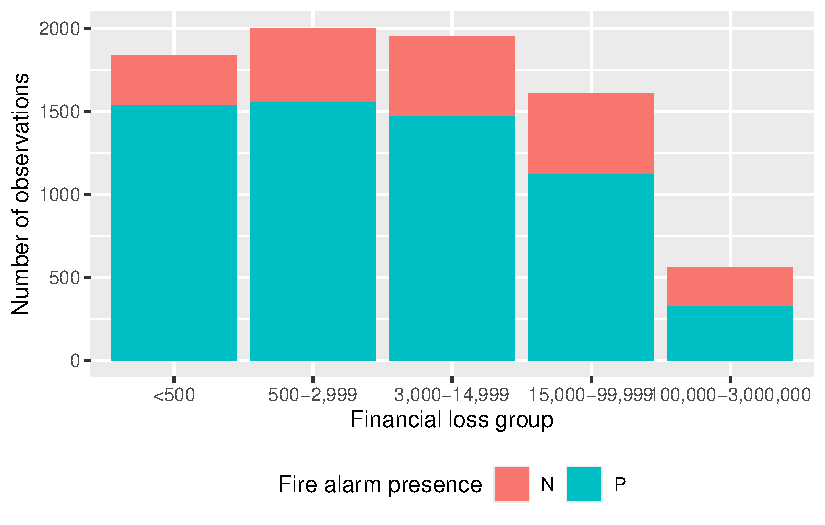
\includegraphics{paper_files/figure-pdf/fig-financial-loss-group-1.pdf}

}

\subcaption{\label{fig-financial-loss-group-1}Distribution of financial
loss group, and fire alarm presence}

\end{minipage}%
%
\begin{minipage}{0.50\linewidth}

\centering{

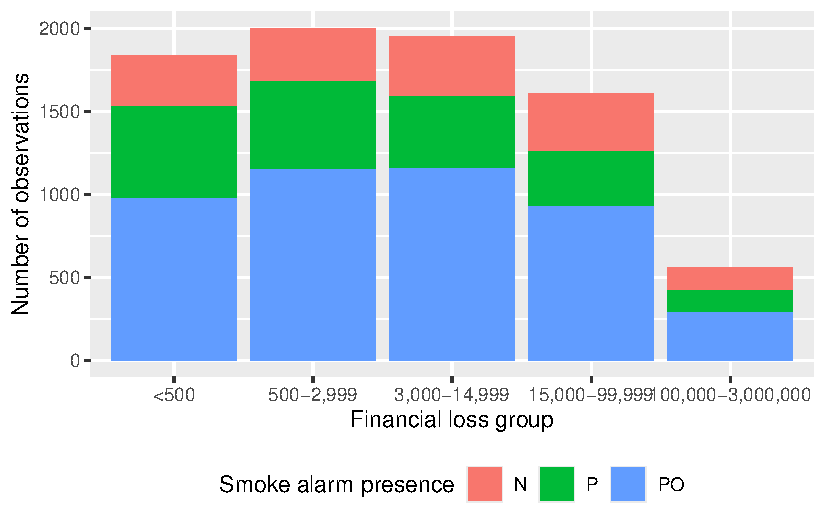
\includegraphics{paper_files/figure-pdf/fig-financial-loss-group-2.pdf}

}

\subcaption{\label{fig-financial-loss-group-2}Distribution of financial
loss group, and smoke alarm presence}

\end{minipage}%
\newline
\begin{minipage}{0.50\linewidth}

\centering{

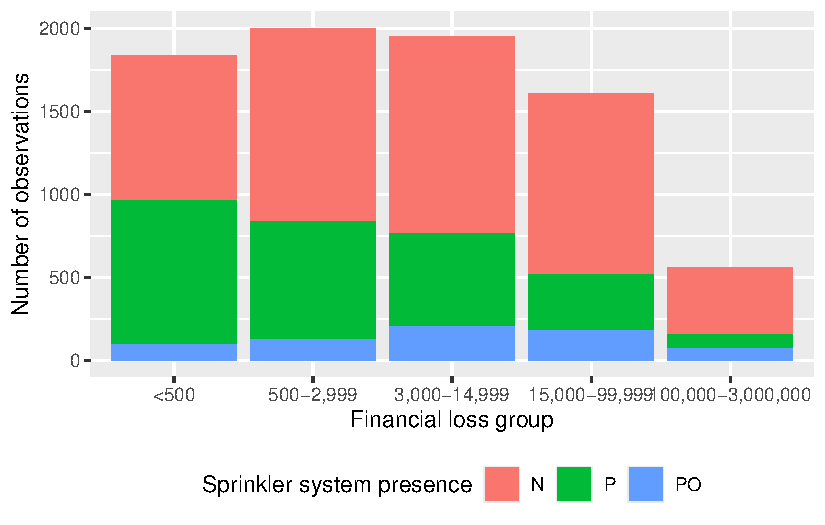
\includegraphics{paper_files/figure-pdf/fig-financial-loss-group-3.pdf}

}

\subcaption{\label{fig-financial-loss-group-3}Distribution of financial
loss group, and sprinkler system presence}

\end{minipage}%

\caption{\label{fig-financial-loss-group}Distribution of financial loss
group, and fire prevention system presence}

\end{figure}%

Figure~\ref{fig-financial-loss-group} shows the distribution of
financial loss in group and the presence of fire prevention system. In
Figure~\ref{fig-financial-loss-group-1}, the graph shows that incidents
with no fire alarm system (red bars) is less than incidents with fire
alarm system (blue bars). Among the incidents with higher financial
loss, there are more cases without fire alarm system. In
Figure~\ref{fig-financial-loss-group-2}, Most of the incidents happen
with the smoke alarm present. Among the incidents with lower financial
loss, more smoke alarms are present but not operated compared to higher
financial loss cases. In Figure~\ref{fig-financial-loss-group-3}, we can
tell that a large proportion of incidents does not have a sprinkler
system installed. Among those incidents with sprinkler system present,
most of them are not operated.

\section{Discussion}\label{discussion}

The analysis of Toronto's fire incident data reveals critical insights
into both the responsiveness of the Toronto Fire Service (TFS) and the
role of fire protection systems in mitigating financial losses.

\subsection{Toronto Fire Service
Responsiveness}\label{toronto-fire-service-responsiveness-1}

The TFS's response times remain generally efficient, with an average
time of approximately 4.9 minutes, as reflected in the summary
statistics (Table~\ref{tbl-clean-tfs-summary-1}). The response time
fluctuated between 5 to 10 minutes over the 2013--2023 period, with some
significant outliers, according to
Figure~\ref{fig-clean-tfs-diff-dollar-time-1}. This suggests that while
TFS generally responds swiftly, occasional delays may occur due to
external factors. The response time does not lead to more financial
loss, because this correlation is weak, as indicated by
Figure~\ref{fig-response-vs-money}. This weak correlation suggests that
it does not matter a lot for the Toronto Fire Service to react to fire
incident very quickly. Other factors, such as the extent of the fire and
fire protection measures in place, play a more critical role in
determining the financial impact of fire incidents.

The financial loss associated with fire incidents shows a wide range,
with most incidents resulting in minimal losses, as shown in
Figure~\ref{fig-clean-tfs-diff-dollar-time-2}. However, some outliers,
particularly between 2015 and 2024, saw losses exceeding \$2 million.
This suggests that there are rare instances where larger fires occur
occasionally, resulting in substantial property damage.

\subsection{Impact of Fire Protection
Equipment}\label{impact-of-fire-protection-equipment}

\newpage

\appendix

\section{Appendix}\label{sec-appendix}

\subsection{Graph of areas of origin of fire incidents by number of
occurrences}\label{sec-origin-fig}

\begin{verbatim}
Index of 'Area of Origin':
\end{verbatim}

\begin{verbatim}
11 - Lobby, Entranceway
12 - Hallway, Corridor
13 - Stairway, Escalator
18 - Covered Court, Atrium, mall concourse
19 - Other Means of Egress
21 - Living Area (e.g. living, TV, recreation, etc)
22 - Sleeping Area or Bedroom (inc. patients room, dormitory, etc)
23 - Dining or Beverage Area (inc mess, canteen, lunchroom, cafeteria
24 - Cooking Area or Kitchen
25 - Washroom or Bathroom (toilet,restroom/locker room)
26 - Sauna
27 - Laundry Area
28 - Office
29 - Electronic Equipment
30 - Sales, Showroom Area
31 - Process Manufacturing (inc manf, prod assembly, repair)
32 - Assembly Area (inc school room,spectator area, church, etc)
33 - Laboratory
34 - Operating Room, Treatment or Examination Area
35 - Performance Area (inc stage, rink, boxing ring, gym floor, altar
36 - Backstage, dressing room
39 - Other Functional Area
41 - Closet (eg. clothes, broom, linen closet, etc.)
42 - Garage
43 - Locker (apartment storage)
44 - Trash, Rubbish Storage (inc garbage chute room, garbage/industri
45 - Supply Storage Room (inc maintenance/office/document storage, et
46 - Product Storage (inc products or materials awaiting manuf, assembly)
47 - Shipping/Receiving/Loading Platform
48 - Records storage area (inc vaults)
49 - Other Storage Area
50 - Basement/cellar (not partitioned)
51 - Elevator (includes shaft)
52 - HVAC Equipment Room (furnace room, water heater closet, boiler)
53 - Chimney/Flue Pipe
54 - Incinerator Room
55 - Mechanical/Electrical Services Room
56 - Conveyor Shaft or Chute (inc dumbwaiter, laundry chute, garbage
57 - Ducting - Heating, Air Conditioning
58 - Ducting - Exhaust (inc cooking, fumes, etc.)
59 - Utility Shaft (eg. electrical wiring/phone, etc.)
60 - Other Building Services/Support Facilities
61 - Exterior Wall
62 - Roof
63 - Awning or Canopy
64 - Porch or Balcony
65 - Crawl Space (includes sub-structure)
66 - Concealed Ceiling Area
67 - Concealed Floor Area
68 - Concealed Wall Area
69 - Attic Area
70 - Other Structural Area
71 - Open Area (inc lawn, field, farmyard, park, playing field, pier,
72 - Court, Patio, Terrace
73 - Parking Area, Parking Lot
74 - Storage Area (outside)
75 - Trash, rubbish area (outside)
78 - Attached Deck
79 - Other Outside Area
81 - Engine Area
82 - Running Gear (inc wheels and braking systems, transmission syste
83 - Electrical Systems
84 - Fuel Systems (eg. fuel tank, etc.)
85 - Operator/Control Area
86 - Passenger Area
87 - Trunk/Cargo Area
89 - Other Vehicle Area
91 - Multiple Areas of Origin
92 - Residential/Business: Restaurant area
93 - Residential/Business: Other busines area
\end{verbatim}

\begin{figure}

\centering{

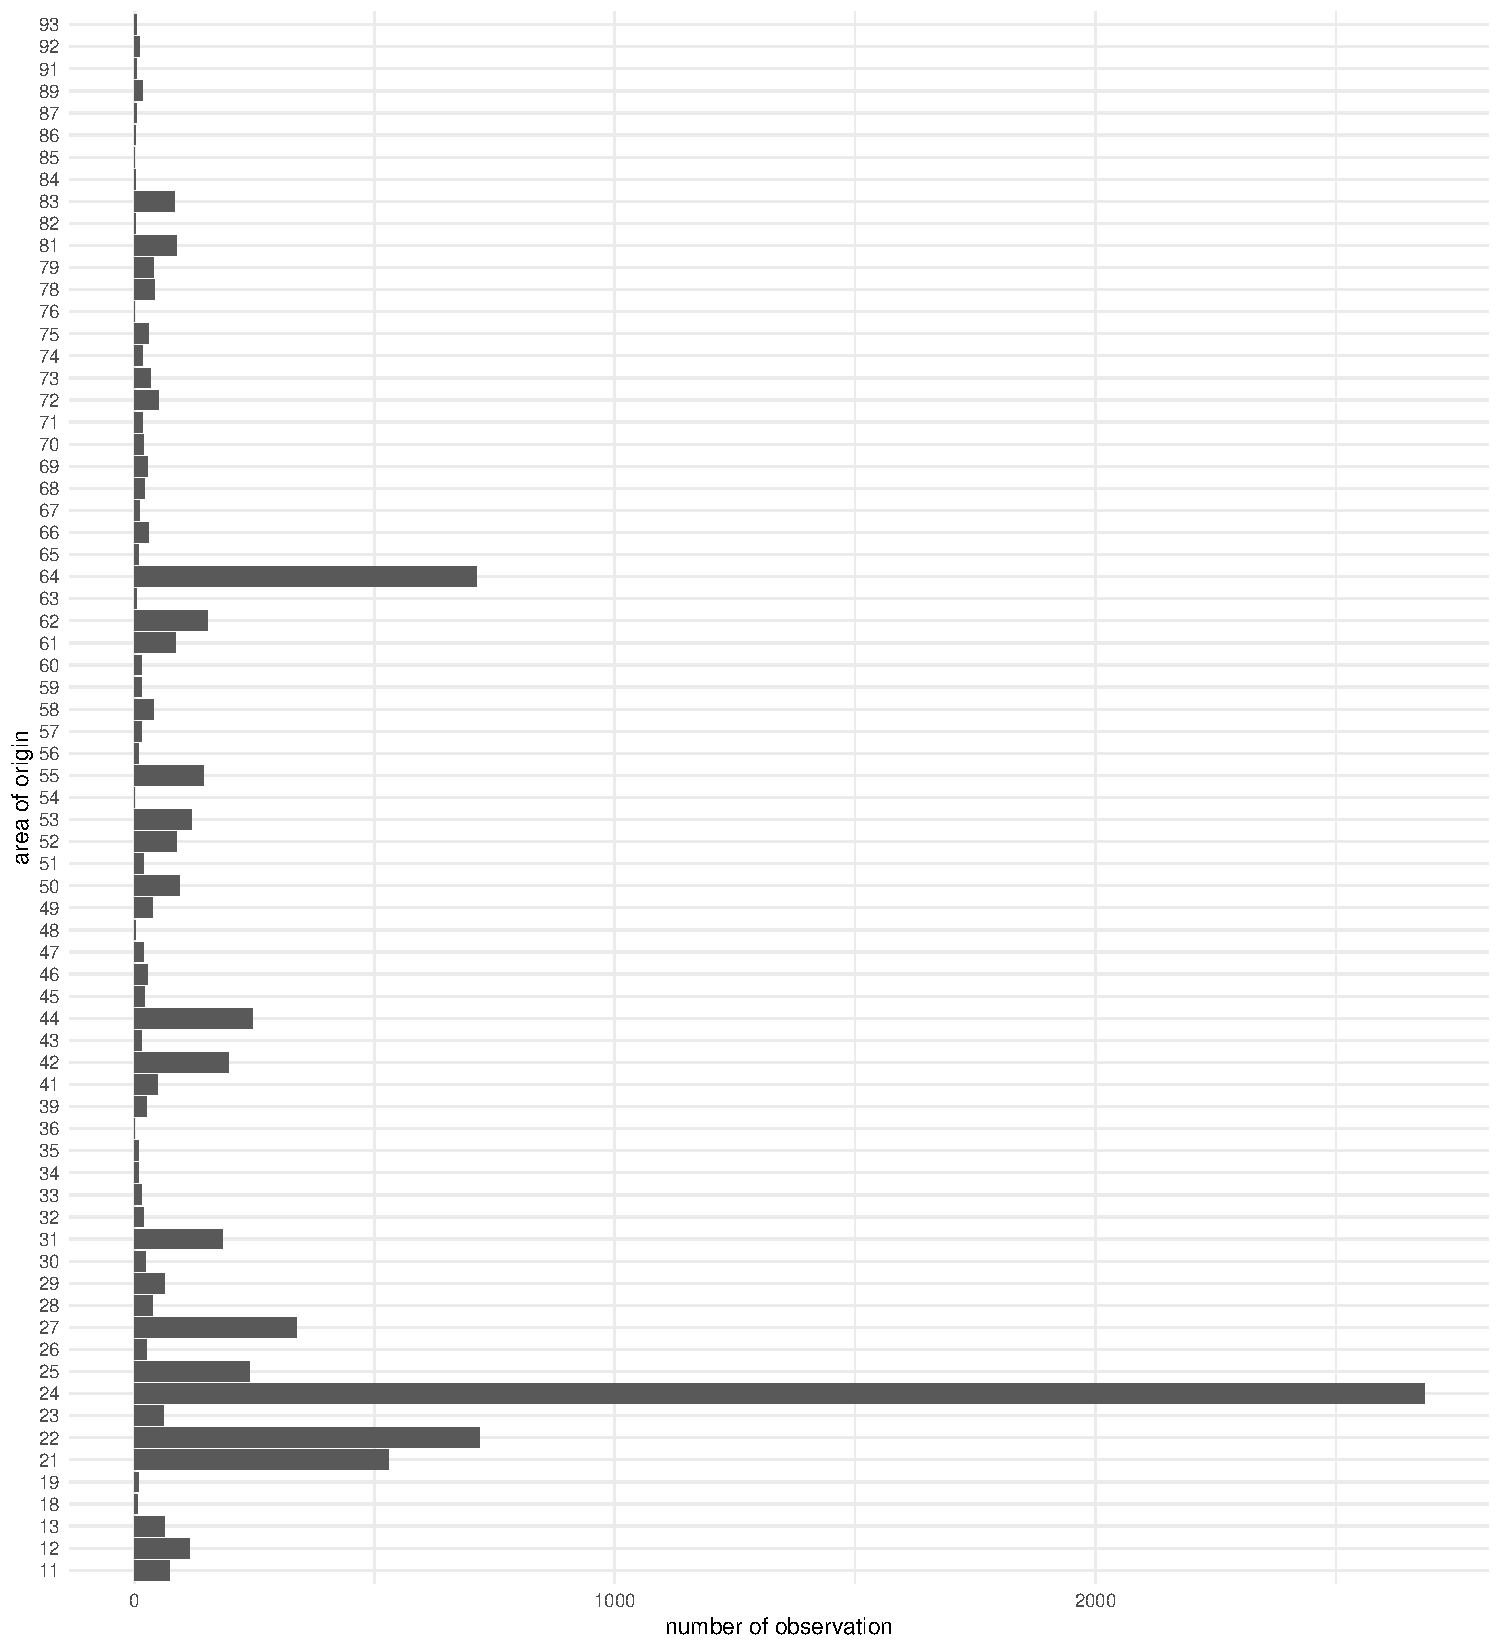
\includegraphics{paper_files/figure-pdf/fig-origin-1.pdf}

}

\caption{\label{fig-origin}Areas of origin of fire incidents by number
of occurrences}

\end{figure}%

\newpage

\subsection{Graph of ignition source of fire incidents by number of
occurrences}\label{sec-source-fig}

\begin{verbatim}
Index of 'Ignition Source':
\end{verbatim}

\begin{verbatim}
100 - Outdoor fireplace/heater
101 - Exposure, source structure detached
102 - Exposure, source structure semi-detached or attached
103 - Exposure, source outside storage container, tank
104 - Exposure, source open fire (inc campfire, rubbish fire)
106 - Exposure, source grass, shrubs, trees
107 - Exposure, source vehicle (outside structure)
108 - Exposure, source other
11 - Stove, Range-top burner
12 - Oven
13 - Microwave
14 - Open Fired Barbeque - Fixed or Portable
15 - Range Hood
16 - Deep Fat Fryer
17 - Wood burning stove
19 - Other Cooking Items (eg Toaster, Kettle, elec frying pan)
20 - Service/Utility Lines (includes power/hydro transmission lines)
21 - Transformer
22 - Meter
23 - Distribution Equipment (includes panel boards, fuses, circuit br
24 - Circuit Wiring - Copper
25 - Circuit Wiring - Aluminum
26 - Terminations-Copper (incl receptacles, switches, lights)
27 - Terminations-Aluminum (incl receptables, switches, lights)
28 - Cord, Cable for Appliance, Electrical Articles
29 - Extension Cord, Temporary Wiring
30 - Other Electrical Distribution Item
31 - Central Heating/Cooling Unit
32 - Water Heater
33 - Space Heater - Fixed
34 - Space Heater - Portable
35 - Fireplace - Factory Built
36 - Fireplace - Masonry
37 - Fireplace Insert
38 - Chimney - Factory Built
39 - Chimney - Masonry
40 - Flue Pipe
41 - Other Heating Equipment
42 - Television, Radio, Stereo, Tape Recorder, etc.
43 - Clothes Dryer
44 - Iron, Pressing Machine
45 - Washing Machine
46 - Electric Blanket, Heating Pad
47 - Refrigerator, Freezer (includes vending machine)
48 - Air Conditioner - Window or Room Unit
49 - Other Appliances
51 - Incandescent Lamp - Light Bulb, Spotlight
52 - Florescent Lamp (includes ballast)
53 - Christmas Lights, Decorative Lighting
54 - Lamp (eg. coal, oil, naphtha, etc.)
55 - Candle
56 - Halogen Lamp or light
59 - Other Lighting Equipment
61 - Incinerator
62 - Heat Treatment Equipment (eg. furnace, oven, kiln, quench tanks,
63 - Painting Equipment
64 - Chemical Processing Equipment (eg. reactors, distilling units, e
69 - Other Processing Equipment
71 - Smoker's Articles (eg. cigarettes, cigars, pipes already ignited
72 - Cutting/Welding Equipment
73 - Blow Torch, Bunsen Burner
74 - Salamander
75 - Matches (open flame)
76 - Lighters (open flame)
77 - Matches or Lighters (unable to distinguish)
79 - Other Open Flame Tools/Smokers' Articles
80 - Portable generator
81 - Vehicle - Electrical
82 - Vehicle - Mechanical
83 - Other Electrical
84 - Other Mechanical
85 - Vehicle collision
88 - Multiple Ignition Source or Igniting Equipment (suspected arson)
91 - Fireworks
92 - Open Fire (eg. camp fire, rubbish fire, etc.)
93 - Hot Ashes, Embers, Spark
94 - Static Electricity (spark)
95 - Lightning
96 - Chemical Reaction (eg. spontaneous combustion, etc.)
97 - Rekindle
\end{verbatim}

\begin{figure}

\centering{

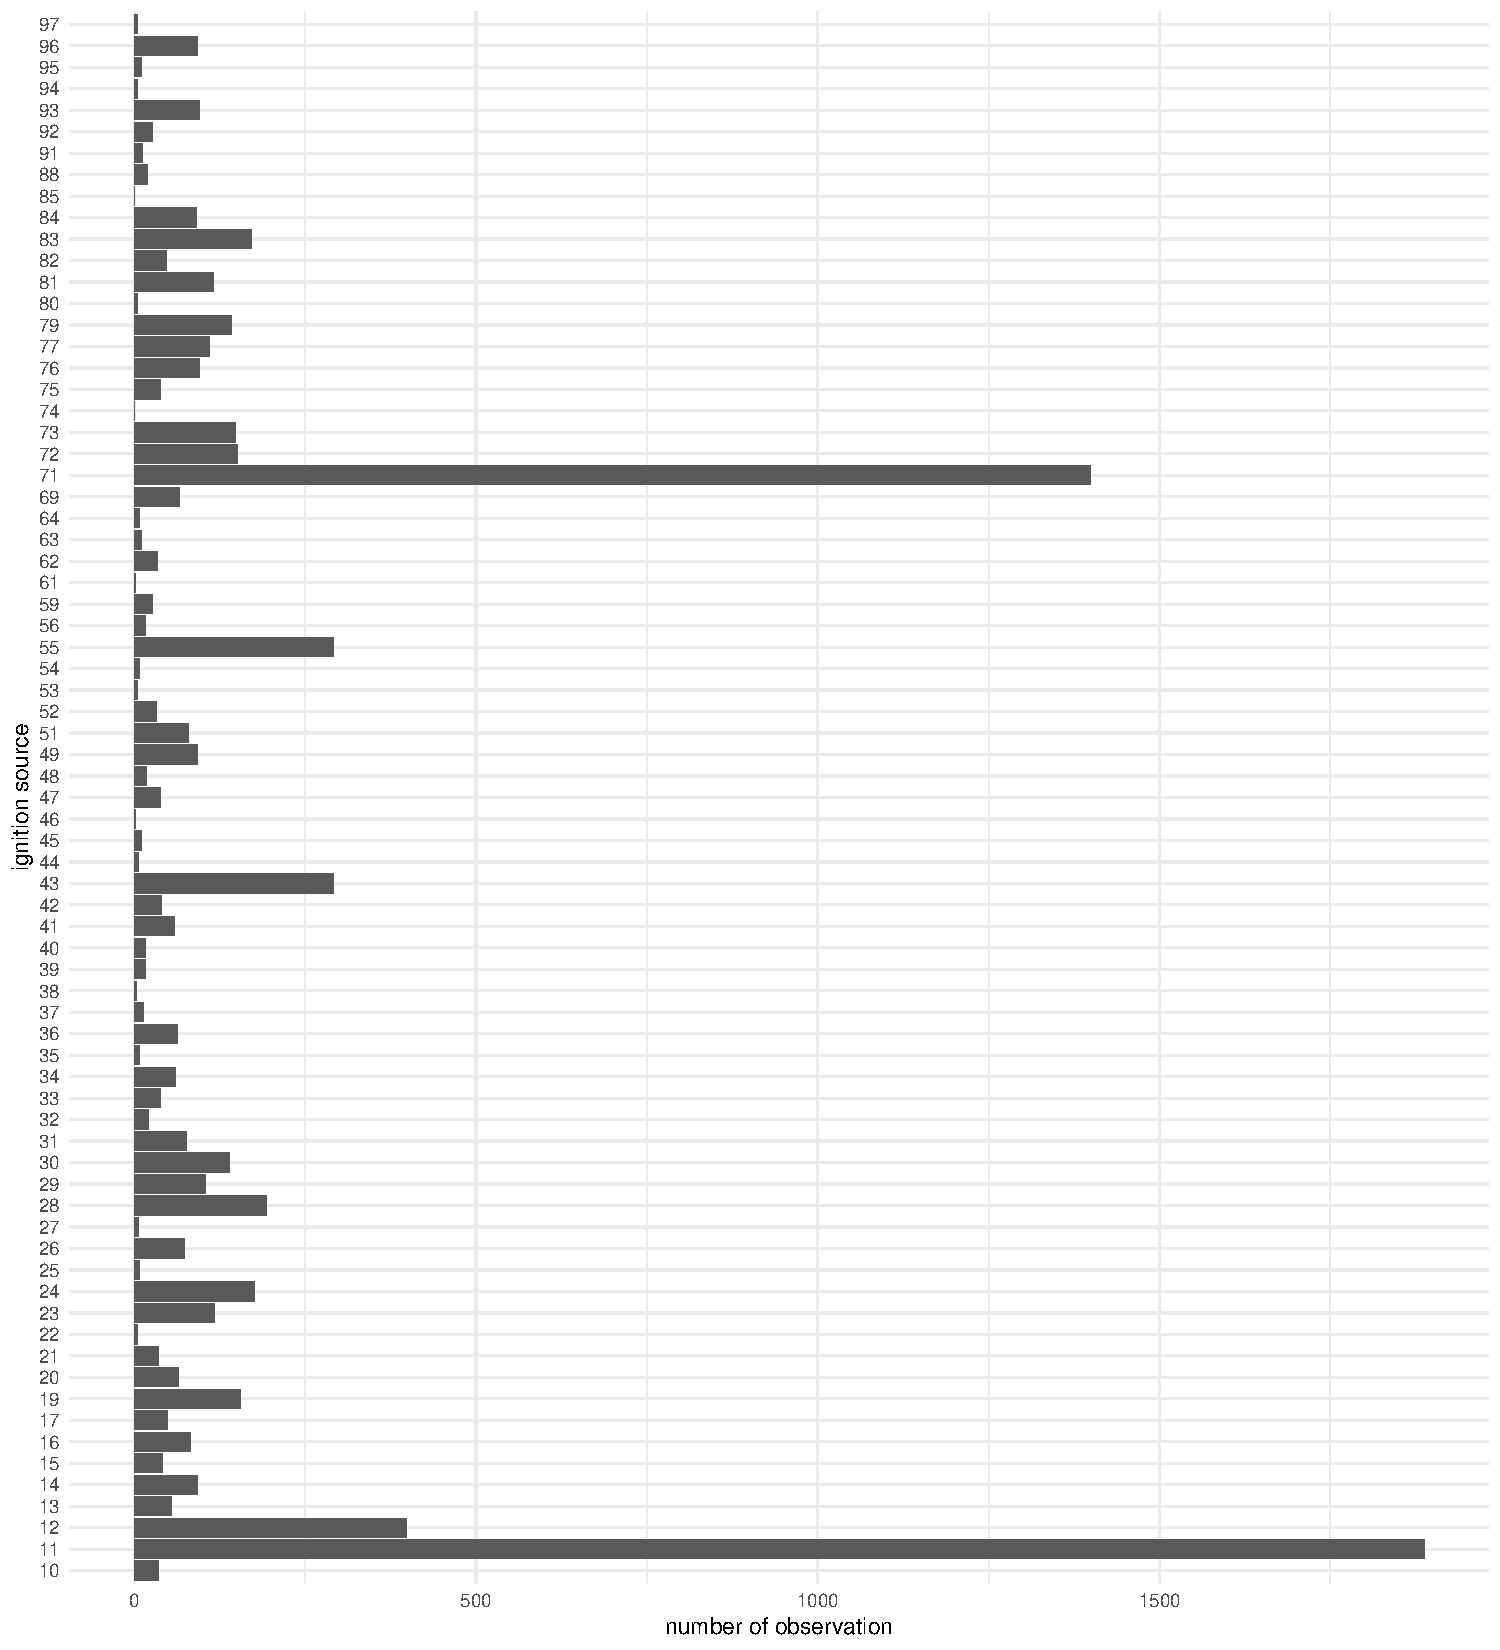
\includegraphics{paper_files/figure-pdf/fig-source-1.pdf}

}

\caption{\label{fig-source}Ignition Source of fire incidents by number
of occurrences}

\end{figure}%

\subsection{Attribution Statement}\label{attribution-statement}

Contains information licensed under the Open Government Licence --
Toronto. Visit: \url{https://open.toronto.ca/open-data-license/}

\newpage

\section*{Bibliography}\label{bibliography}
\addcontentsline{toc}{section}{Bibliography}

\phantomsection\label{refs}
\begin{CSLReferences}{1}{0}
\bibitem[\citeproctext]{ref-opendatatoronto}
Gelfand, Sharla. 2022. \emph{Opendatatoronto: Access the City of Toronto
Open Data Portal}.
\url{https://CRAN.R-project.org/package=opendatatoronto}.

\bibitem[\citeproctext]{ref-Goemans2012}
Goemans, Magdalene, and Patricia Ballamingie. 2012. {``Forest as Hazard,
Forest as Victim: Community Perspectives and Disaster Mitigation in the
Aftermath of Kelowna's 2003 Wildfires.''} \emph{Canadian Geographies /
Géographies Canadiennes} 57 (1): 56--71.
\url{https://doi.org/10.1111/j.1541-0064.2012.00447.x}.

\bibitem[\citeproctext]{ref-lubridate}
Grolemund, Garrett, and Hadley Wickham. 2011. {``Dates and Times Made
Easy with {lubridate}.''} \emph{Journal of Statistical Software} 40 (3):
1--25. \url{https://www.jstatsoft.org/v40/i03/}.

\bibitem[\citeproctext]{ref-HariMurti2023}
Hari Murti, Raditya, Hendra Adi Wijaya, Indira Laksmi Widuri, Julmadian
Abda, Mada Sophianingrum, Muhammad Rizki Islami, Ahady Farrel
Febriyanto, and Eduardo Erlangga Drestanta. 2023. {``Risk Assessment of
Fire Hazards in Semarang City Residential Areas.''} \emph{Jurnal Teknik
Sipil Dan Perencanaan} 25 (1): 52--61.
\url{https://doi.org/10.15294/jtsp.v25i1.42955}.

\bibitem[\citeproctext]{ref-Mamuji2018}
Mamuji, Aaida A., and Jack L. Rozdilsky. 2018. {``Wildfire as an
Increasingly Common Natural Disaster Facing Canada: Understanding the
2016 Fort McMurray Wildfire.''} \emph{Natural Hazards} 98 (1): 163--80.
\url{https://doi.org/10.1007/s11069-018-3488-4}.

\bibitem[\citeproctext]{ref-MasoodRafi2012}
Masood Rafi, Muhammad, Syed Wasiuddin, and Salman Hameed Siddiqui. 2012.
{``Assessment of Fire Hazard in Pakistan.''} \emph{Disaster Prevention
and Management: An International Journal} 21 (1): 71--84.
\url{https://doi.org/10.1108/09653561211202719}.

\bibitem[\citeproctext]{ref-citeR}
R Core Team. 2024. \emph{R: A Language and Environment for Statistical
Computing}. Vienna, Austria: R Foundation for Statistical Computing.
\url{https://www.R-project.org/}.

\bibitem[\citeproctext]{ref-statsCanada}
Statistics Canada. 2024. {``Components of Population Change by Census
Metropolitan Area and Census Agglomeration, 2021 Boundaries.''}
Government of Canada. \url{https://doi.org/10.25318/1710014901-ENG}.

\bibitem[\citeproctext]{ref-ggplot2}
Wickham, Hadley. 2016. \emph{Ggplot2: Elegant Graphics for Data
Analysis}. Springer-Verlag New York.
\url{https://ggplot2.tidyverse.org}.

\bibitem[\citeproctext]{ref-tidyverse}
Wickham, Hadley, Mara Averick, Jennifer Bryan, Winston Chang, Lucy
D'Agostino McGowan, Romain François, Garrett Grolemund, et al. 2019.
{``Welcome to the {tidyverse}.''} \emph{Journal of Open Source Software}
4 (43): 1686. \url{https://doi.org/10.21105/joss.01686}.

\bibitem[\citeproctext]{ref-dplyr}
Wickham, Hadley, Romain François, Lionel Henry, Kirill Müller, and Davis
Vaughan. 2023. \emph{Dplyr: A Grammar of Data Manipulation}.
\url{https://CRAN.R-project.org/package=dplyr}.

\bibitem[\citeproctext]{ref-knitr}
Xie, Yihui. 2014. {``Knitr: A Comprehensive Tool for Reproducible
Research in {R}.''} In \emph{Implementing Reproducible Computational
Research}, edited by Victoria Stodden, Friedrich Leisch, and Roger D.
Peng. Chapman; Hall/CRC.

\end{CSLReferences}




\end{document}
